\chapter{Fichier additionnel associé au chapitre \ref{chapter:gwena}}
\label{annexe:supp_file_GWENA}

\begin{center}
{\huge Additional file 1}\\
\hfill \break
{\large GWENA: gene co-expression networks analysis and extended modules characterization in a single Bioconductor package} \\ 
\hfill \break
\textit{Gwenaëlle G. Lemoine, Marie-Pier Scott-Boyer, Bathilde Ambroise, Olivier Périn, Arnaud Droit}
\end{center}


%% ++++++++++++++++++++++++++++++++++++++++++++++++++++++++++++++++++++++++++++++++++++
%% +                    Z summary & combination NetRep                                +
%% ++++++++++++++++++++++++++++++++++++++++++++++++++++++++++++++++++++++++++++++++++++
\section{Supplementary Material and Method}
\subsection{Z summary detail and combination with NetRep}
\label{supp:supp_z_summary_detail}

As NetRep uses a permutation test with the null hypothesis of the module being not preserved, it can only return if the module is preserved or not significant. To determine if a module is not preserved or moderately preserved, a Z summary statistic is computed using the topological metrics defined by Langfelder et al. \cite{Langfelder2011} and renamed by NetRep \cite{Ritchie2016} such as : \\

\[Z_{summary} = \frac{Z_{density} + Z_{connectivity}}{2}\] \\

\begin{figure}[ht]
    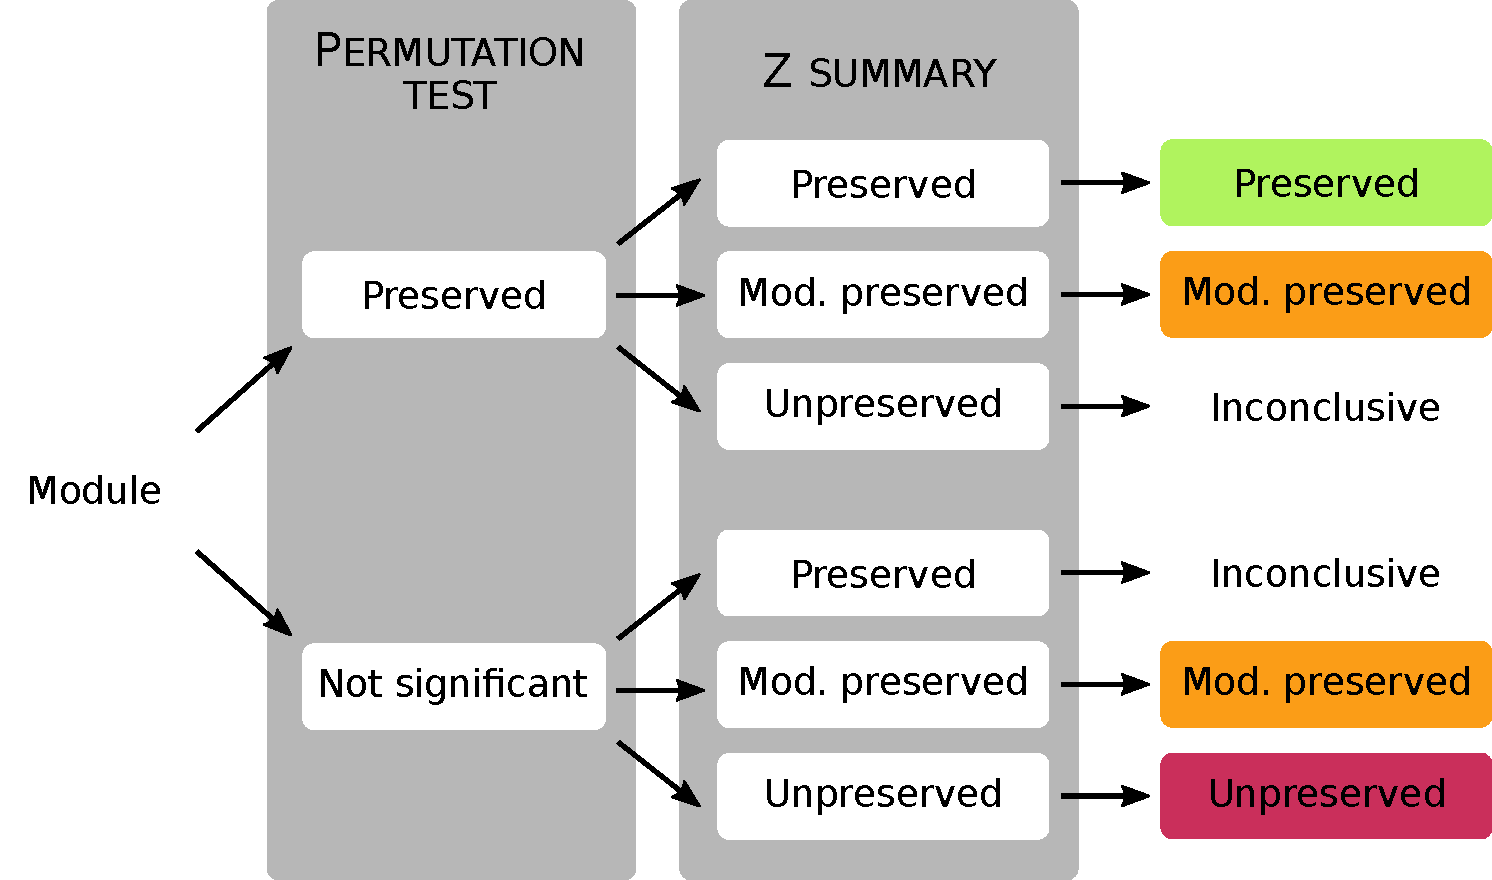
\includegraphics[width=\textwidth, center]{img/annexe_add_file_GWENA/additional_file_figure_1.pdf}
    \caption{Combination of the permutation test result ans the $Z_{summary}$ result in GWENA to return a final result on the module comparison.}
    \label{fig:supp_fig_comparison_schema_conclusion}
\end{figure}


With the NetRep notation :
\begin{align*}
    Z_{density} & = median(Z_{cor.density},Z_{avg.edge.wei},Z_{mod.coh},Z_{avg.node.contrib}) \\
    Z_{connectivity} & = median(Z_{concor.wei.deg},Z_{concor.nod.contrib},Z_{concor.cor})
\end{align*} 

Where : 
\begin{small}
    \begin{align*}
        cor.density & = \text{mean}(vect.Matrix(\text{sign}(r_{ij}^{[ref](q)}r{ij}^{[test](q)})))    & vect.Matrix(A) & = (a_{2,1},a_{3,1},...,a_{n,1},a_{n,n-1}) \\
        avg.edge.wei & = density^{[test](q)} = \text{mean}(vect.Mat(A^{[test](q)}))        & r_{ij}^{[ref]} & = \text{cor}(x_i^{[ref]}, x_j^{[ref]})\\
        mod.coh & = \text{mean}_{i\in Mq}((kME_i^{[test](q)})^2)        & r_{ij}^{[test]} & = \text{cor}(x_i^{[test]}, x_j^{[test]})\\
        avg.node.contrib & = \text{mean}_{i\in Mq}(\text{sign}(kME_i^{[ref](q)})kME_i^{[test](q)})  \\
        concor.wei.deg & = \text{cor}(kIM)^{[ref](q)}, kIM^{[test](q)}  \\
        concor.nod.contrib & = \text{cor}_{i\in Mq}(kME_i^{[ref](q)},kME_i^{[test](q)})  \\
        concor.cor & = \text{cor}(vect.Matrix(r^{[ref](q)}), vect.Matrix(r^{[test](q)}))  
    \end{align*}
\end{small}

This score returns :
\begin{itemize}
    \item \textbf{Preserved} if the $Z_{summary}$ is above 10
    \item \textbf{Moderately preserved} if the $Z_{summary}$ is between 2 and 10
    \item \textbf{Unpreserved} if the $Z_{summary}$ is below 2
\end{itemize} 

\hfill\break

The results from both NetRep permutation test and the $Z_{summary}$ are then combined in GWENA as shown in Figure \ref{fig:supp_fig_comparison_schema_conclusion} and return a final result on the module comparison.


%% ++++++++++++++++++++++++++++++++++++++++++++++++++++++++++++++++++++++++++++++++++++
%% +                                    Details data                                  +
%% ++++++++++++++++++++++++++++++++++++++++++++++++++++++++++++++++++++++++++++++++++++



\subsection{Details on case study data}
\label{supp:supp_detail_data_software}

Public data were obtained from GTEx v8 version on the GTEx Portal on 09/20/2020. 
Access to private data was subject to a request to dbGaP on accession number phs000424.v8.p2. Data were obtained on 10/21/2020.

\begin{table}[h!]
\begin{tabular}{ll}
\textbf{Data}      & \textbf{File}                                                     \\ \hline
Gene expression    & GTEx\_Analysis\_2017-06-05\_v8\_RNASeQCv1.1.9\_gene\_reads.gct.gz \\
Public annotation  & GTEx\_Analysis\_v8\_Annotations\_SampleAttributesDS.txt           \\
Private annotation & phs000424.v8.pht002742.v8.p2.c1.GTEx\_Subject\_Phenotypes.GRU.txt \\
Phenotype          & GTEx\_Analysis\_v8\_Annotations\_SubjectPhenotypesDS.txt         
\end{tabular}
\caption{Correspondence between file names and their contents}
\end{table}



%% ++++++++++++++++++++++++++++++++++++++++++++++++++++++++++++++++++++++++++++++++++++
%% +                                  PC-correction                                   +
%% ++++++++++++++++++++++++++++++++++++++++++++++++++++++++++++++++++++++++++++++++++++


\subsection{GTEx data normalization with PC-correction method}
\label{supp:supp_pc_correction}

In order to limit batch effect and handle the maximum of other co-founding effects, we chose to use a method based on PC-correction as recommended by Parsana et al. \cite{Parsana2019} for GTEx data. However age is usually included in this confounding factors, therefore is corrected. Since we're interested in gene changes we adapted the method to remove only the top $n$ PC correlated to age and which removed the least of genes correlating with age. The $n$ number of PC to remove was estimated by calculating the loss of correlation between phenotype and genes expression (Figure \ref{fig:supp_fig_ageing_correlation_density}) and confirmed by looking for the number of significantly correlated genes with two ageing gene databases (Figure \ref{fig:supp_fig_ageing_genes_overlapping}): GenAge \cite{Tacutu2018} and Digital Aging Atlas \cite{Craig2015}.

\begin{figure}[ht]
    % \centering
    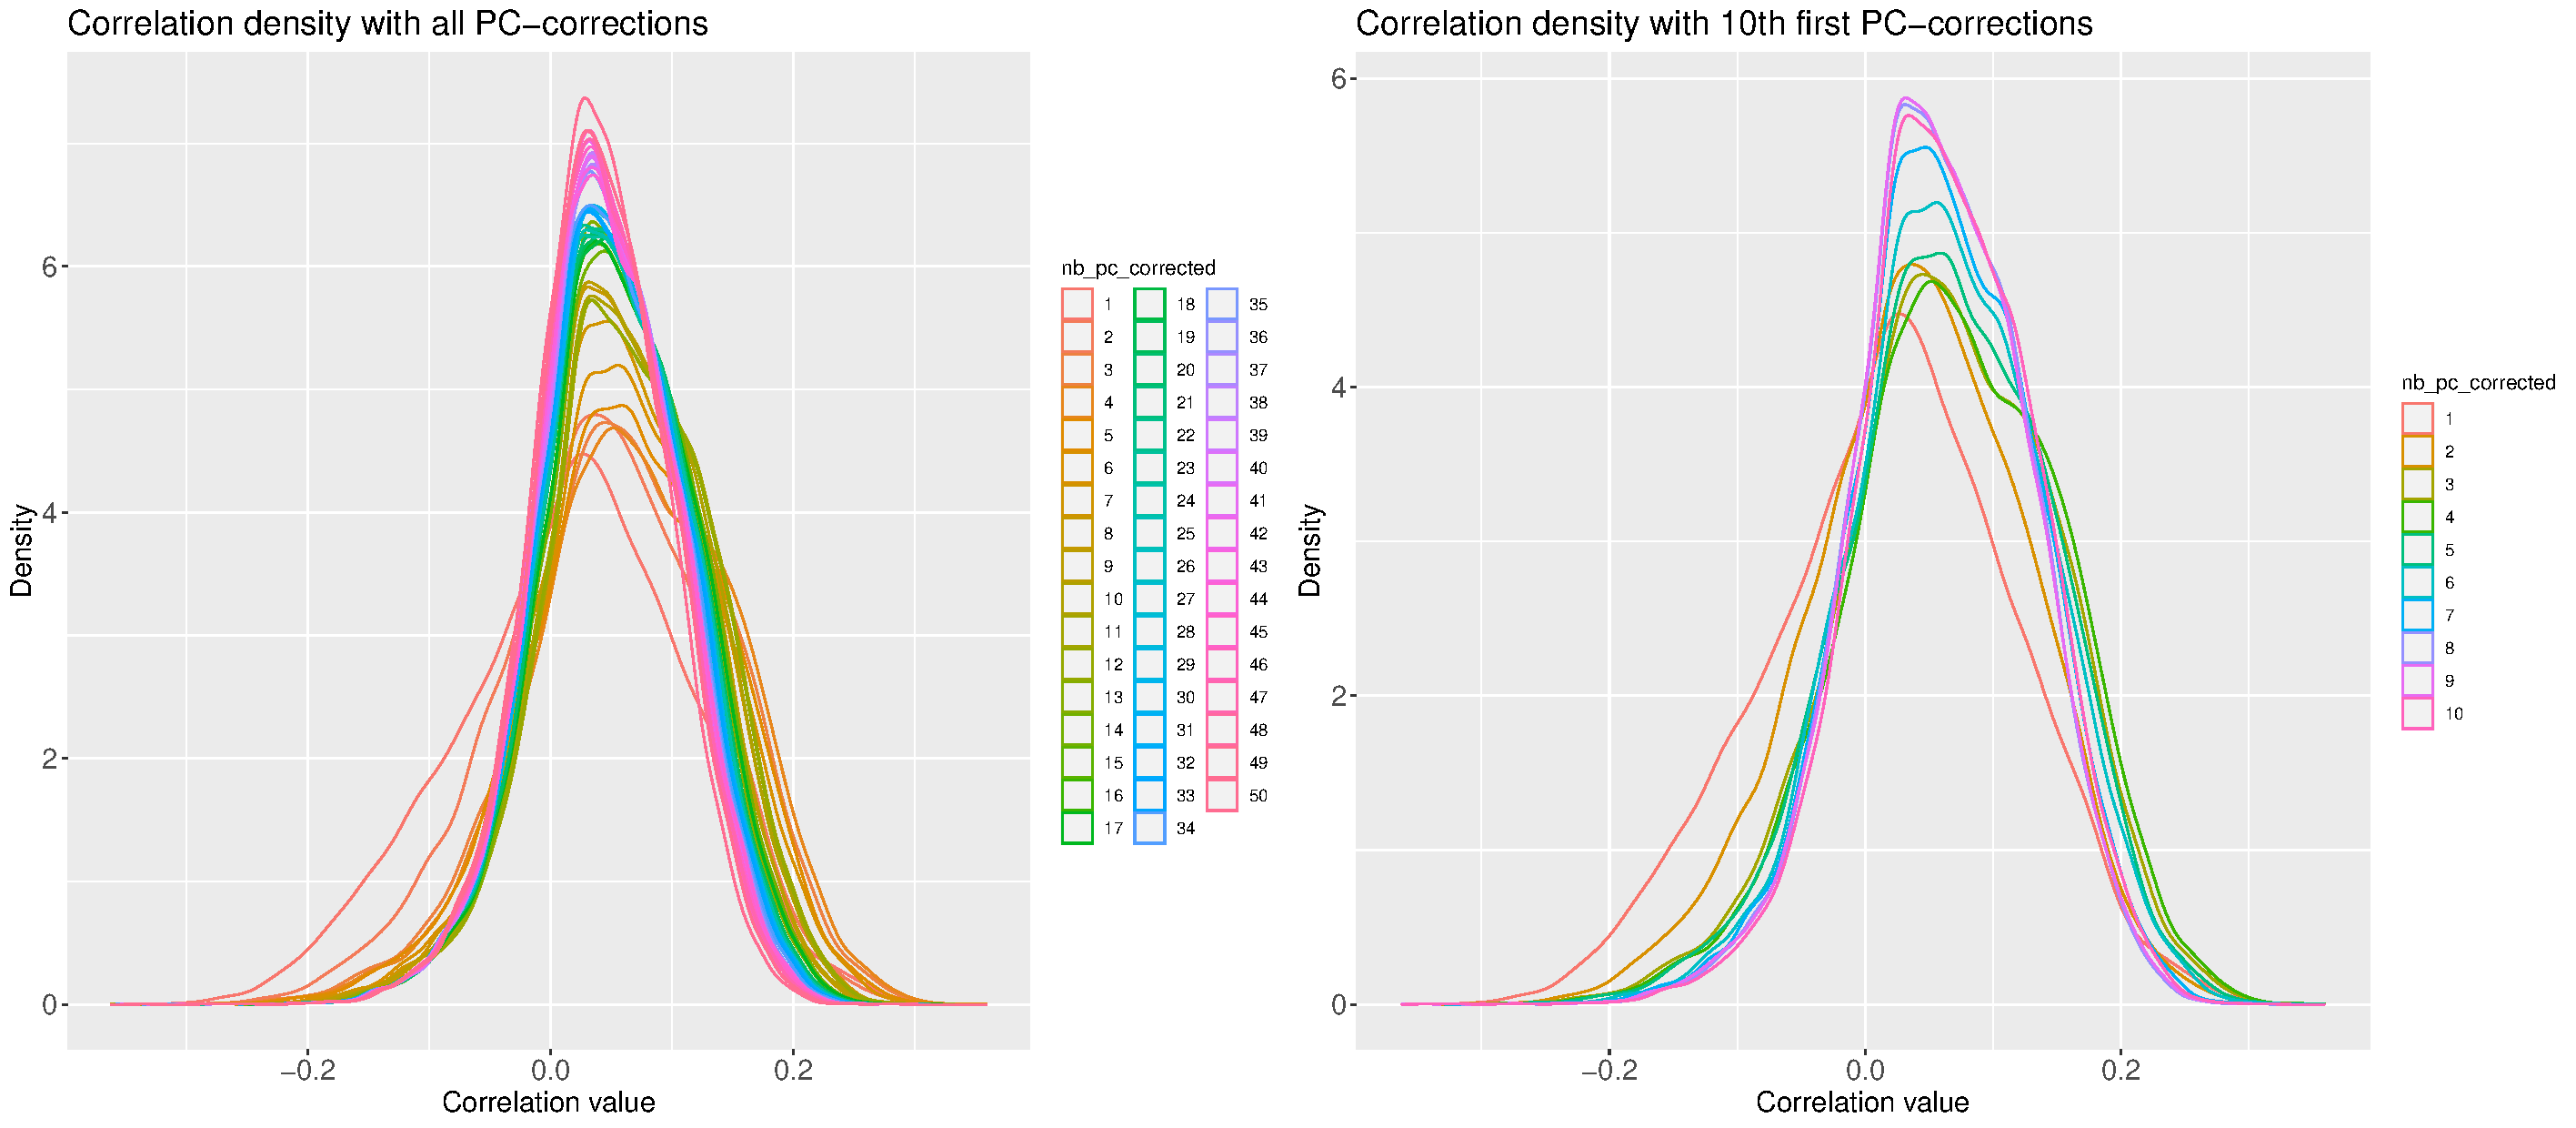
\includegraphics[width=\textwidth, center]{img/annexe_add_file_GWENA/additional_file_figure_2.pdf}
    \caption{Ageing genes correlation density with phenotype depending on the number of PC corrected. Left figure contains all PC correction tested. For clarity we filtered on the first 10 PC corrected on the right figure.}
    \label{fig:supp_fig_ageing_correlation_density}
\end{figure}

\begin{figure}[ht]
    % \centering
    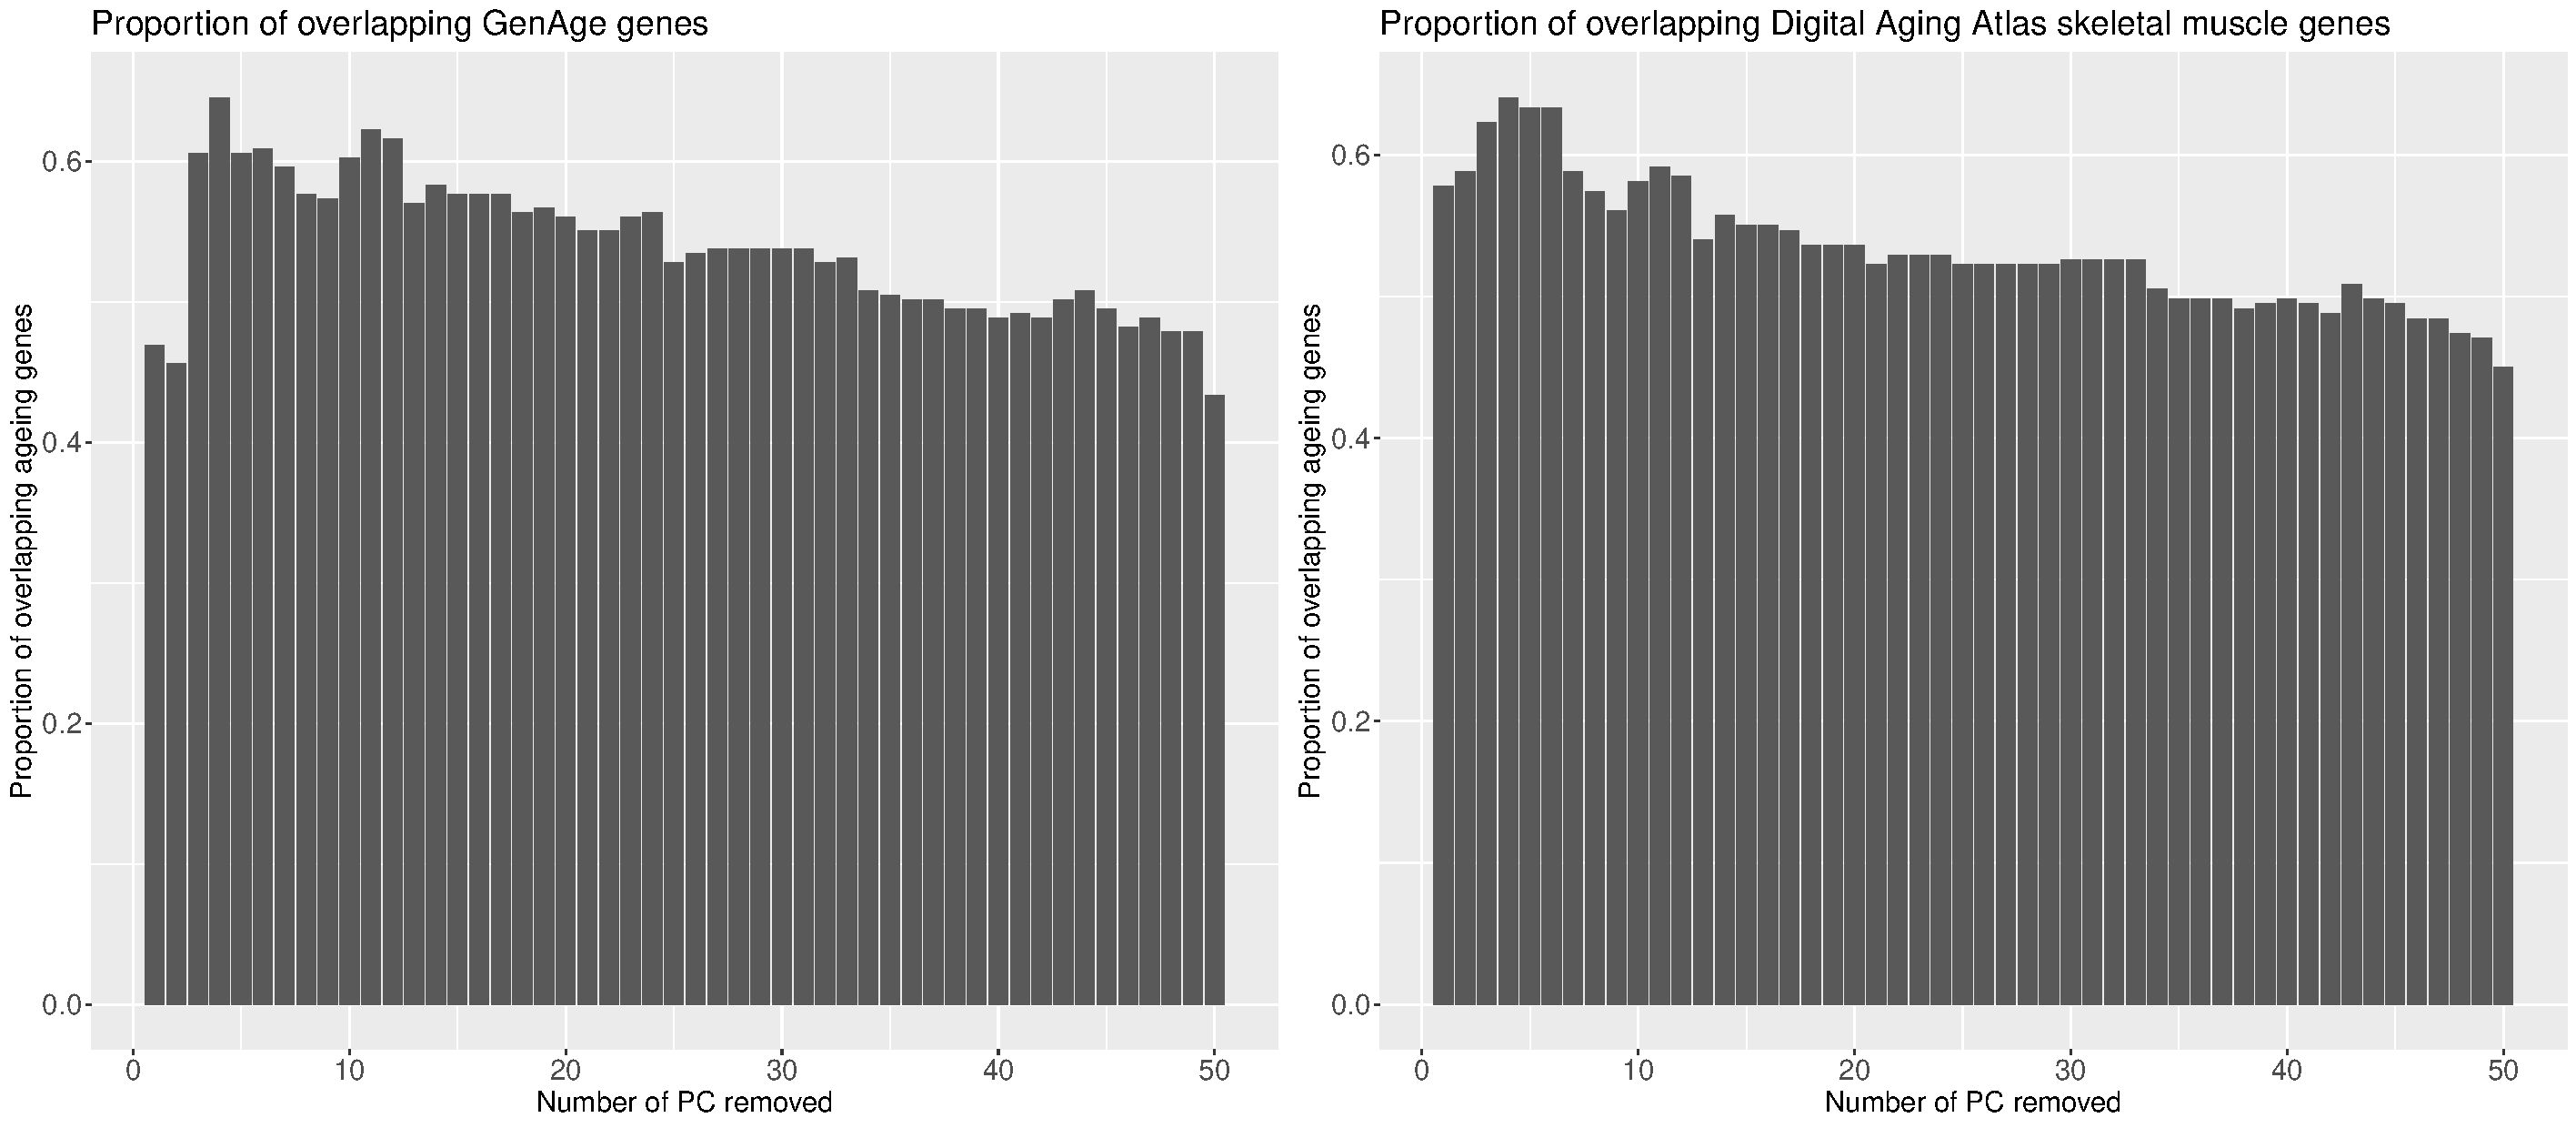
\includegraphics[width=\textwidth, center]{img/annexe_add_file_GWENA/additional_file_figure_3.pdf}
    \caption{Number of genes known to be associated with ageing.}
    \label{fig:supp_fig_ageing_genes_overlapping}
\end{figure}

Correlation density in Figure \ref{fig:supp_fig_ageing_correlation_density} suggest a similarity between the corrections from 2 to 5 PC removal. Combined with the proportion of overlapping known ageing genes in Figure \ref{fig:supp_fig_ageing_genes_overlapping} we determined the optimal number of PC $n$ to remove to be 4.

\clearpage
\section{Supplementary Results}
\subsection{Connectivity drop on all modules}
\label{supp:supp_connectivity_drop}

\begin{figure}[hb]
    \begin{adjustbox}{addcode=
        {\begin{minipage}{\width}}
        {
                \caption{Distribution of the connectivity for each gene by module between the two age range. Genes connectivity is ordered by increasing connectivity in the young condition (red).}
            \end{minipage}
        },rotate=90,center}
        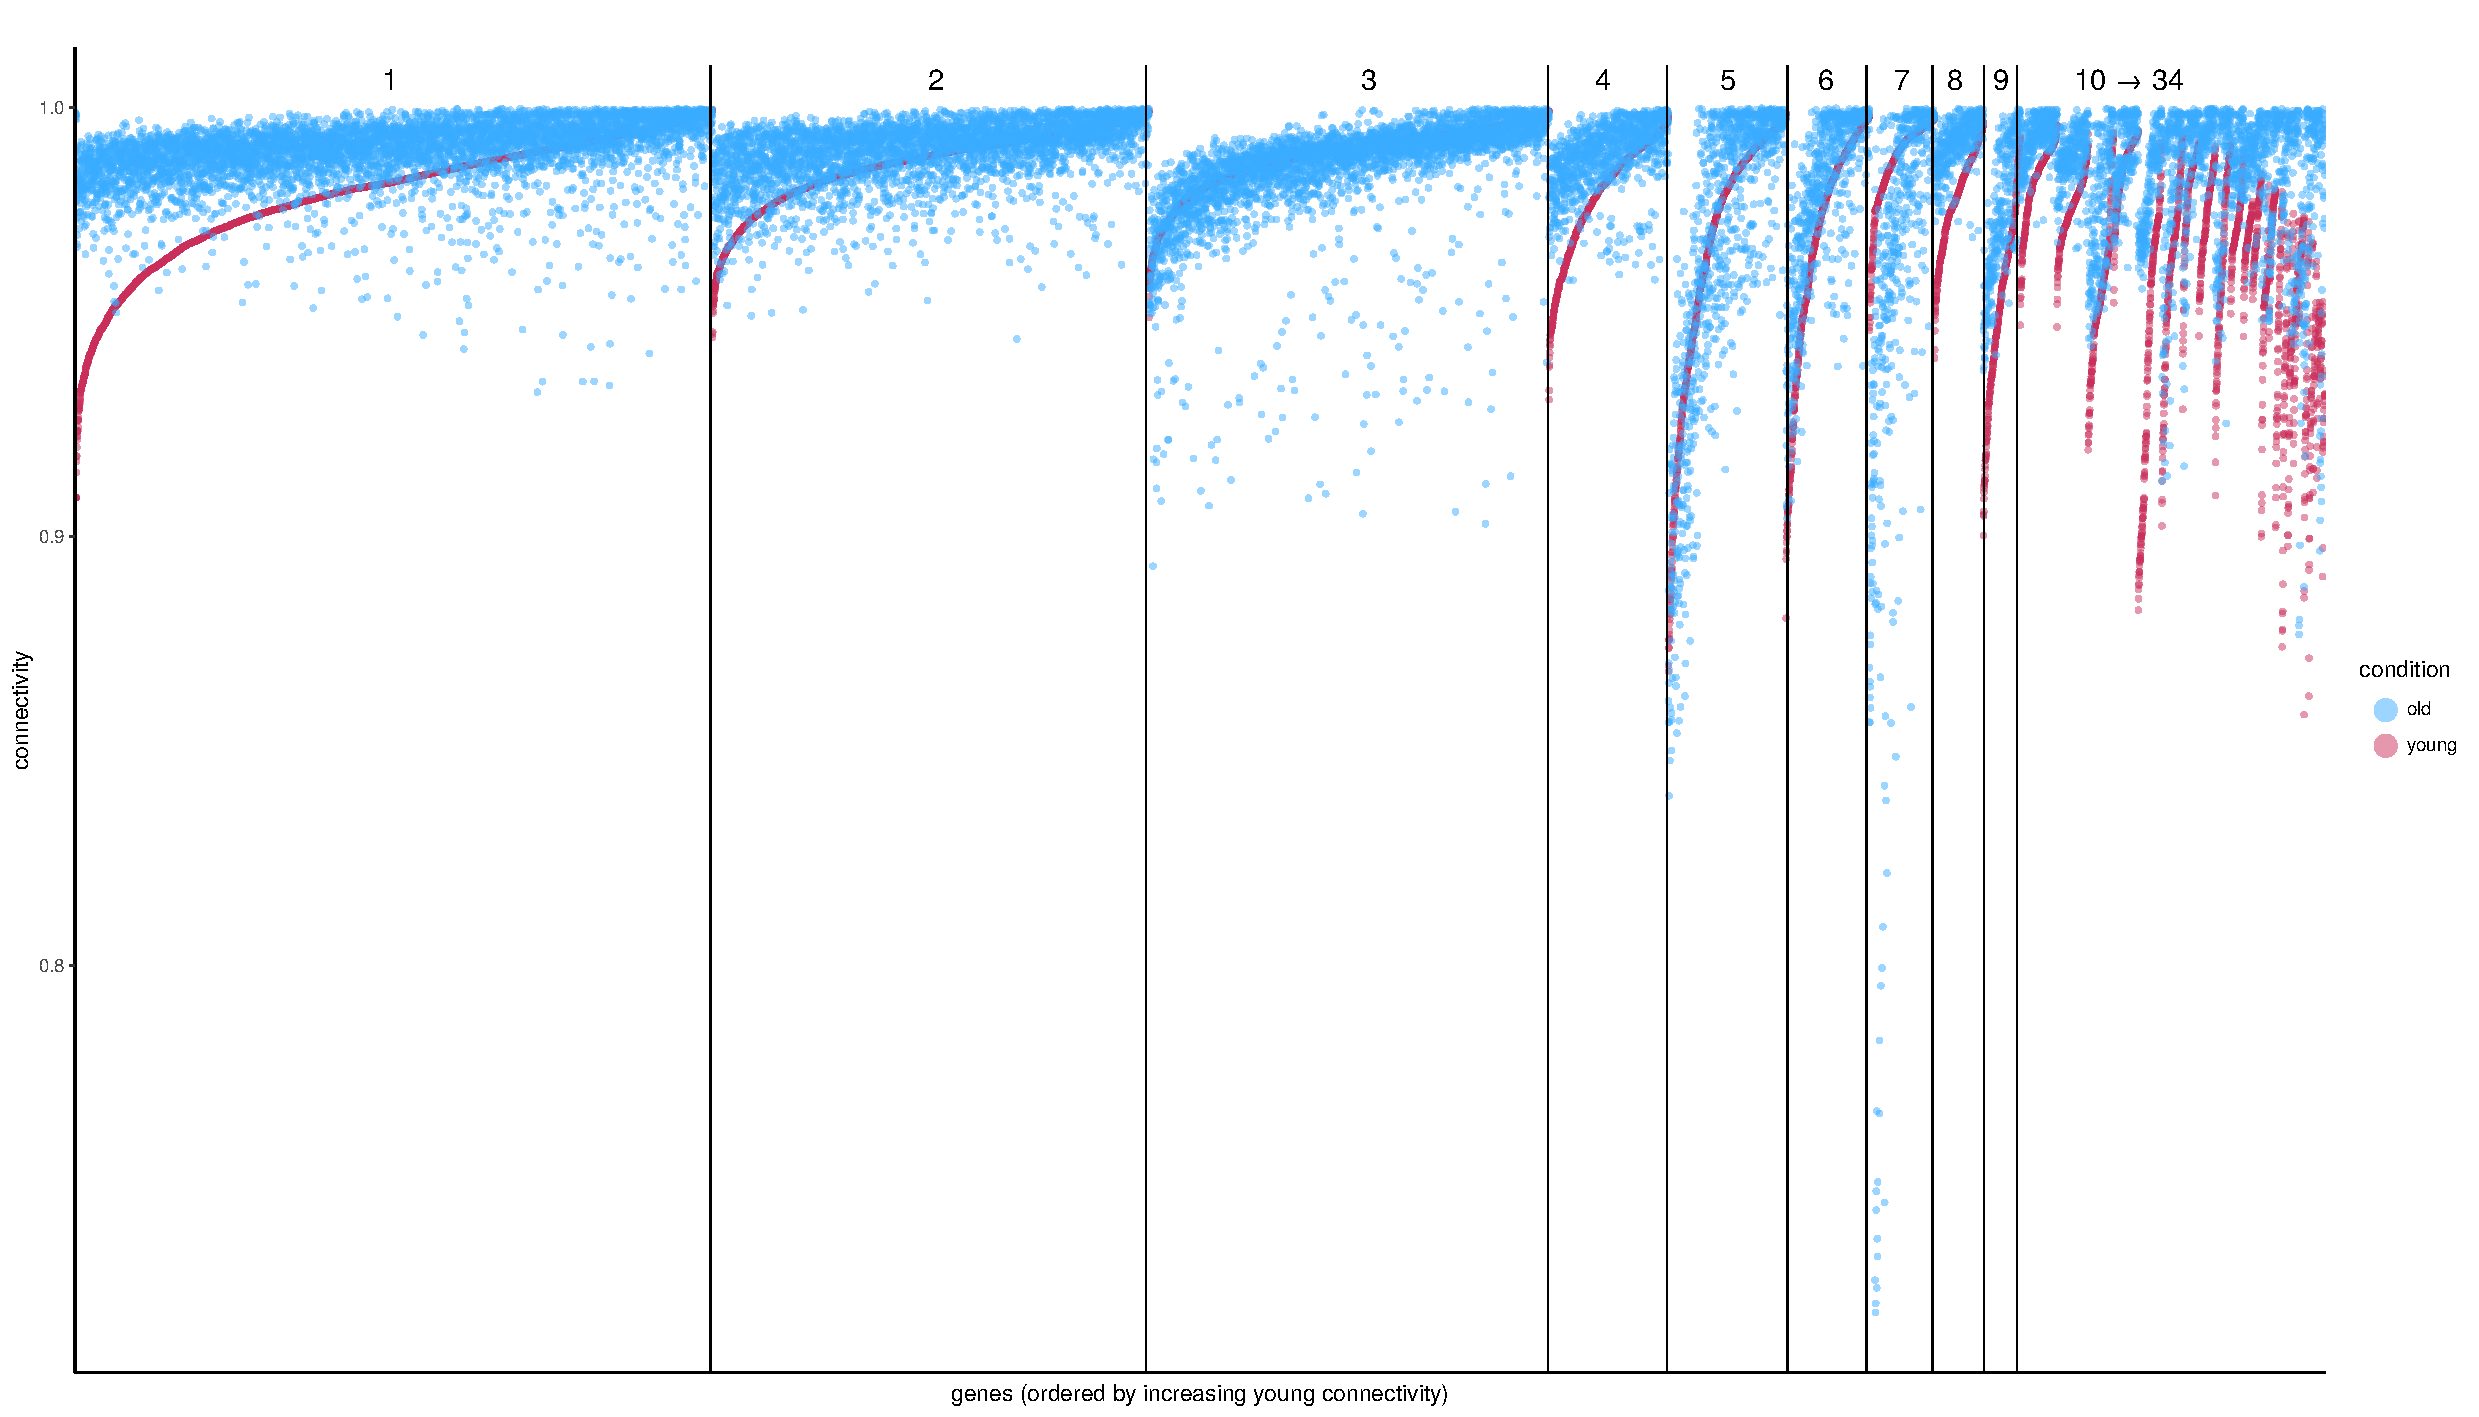
\includegraphics[scale=.476]{img/annexe_add_file_GWENA/additional_file_figure_4.pdf}%
    \end{adjustbox}
\end{figure}

\clearpage
\subsection{New enrichment terms in sub module 6 from module 7 old age range}
\label{supp:supp_sub_cluster_6_enrich_table}

% \resizebox{\textwidth}{!}{ % gneu gneu gneu marche pas
\LTcapwidth=\textwidth
% \setlength\LTright{3pt}
% \setlength\LTleft{0pt}
\begin{longtable}{@{}lp{5cm}lllp{5cm}l@{}}
\caption[Enrichment table from module 7 sub module 6 in old condition]{Enrichment table from module 7 sub module 6 in old condition. Terms are sorted along their novelty (is the enrichment new compared to the enrichments from sub modules in the young age range) and then the source. Source is the enrichment database used on the gene set (GO:BP = Gene Ontology : Biological Process, GO:CC = Gene Ontology Cellular Compartment, GO:MF = Gene Ontology : Molecular Function, HP : Human Phenotype Ontology, WP = WikiPathway, KEGG = Kyoto Encyclopedia of Genes and Genomes, REAC = Reactome, TF = Transfac).}
\\ \hline
\textbf{source} & \textbf{term name}                                                                                                                & \textbf{is new} & \textbf{} & \textbf{source} & \textbf{term name}                                                                                                                                                    & \textbf{is new} \\ \hline
CORUM           & Fibrinogen complex                                                                                                                 & no               &           & GO:BP           & regulation of vasoconstriction                                                                                                                                         & yes              \\
GO:BP           & fibrinolysis                                                                                                                       & no               &           & GO:BP           & heterotypic cell-cell adhesion                                                                                                                                         & yes              \\
GO:BP           & negative regulation of blood coagulation                                                                                           & no               &           & GO:BP           & platelet aggregation                                                                                                                                                   & yes              \\
GO:BP           & negative regulation of hemostasis                                                                                                  & no               &           & GO:BP           & regulation of endothelial cell apoptotic process                                                                                                                       & yes              \\
GO:BP           & negative regulation of coagulation                                                                                                 & no               &           & GO:BP           & endothelial cell apoptotic process                                                                                                                                     & yes              \\
GO:BP           & negative regulation of wound healing                                                                                               & no               &           & GO:BP           & protein processing                                                                                                                                                     & yes              \\
GO:BP           & negative regulation of response to wounding                                                                                        & no               &           & GO:BP           & cell-matrix adhesion                                                                                                                                                   & yes              \\
GO:BP           & regulation of body fluid levels                                                                                                    & no               &           & GO:BP           & positive regulation of response to wounding                                                                                                                            & yes              \\
GO:CC           & blood microparticle                                                                                                                & no               &           & GO:BP           & positive regulation of blood circulation                                                                                                                               & yes              \\
GO:CC           & platelet alpha granule lumen                                                                                                       & no               &           & GO:BP           & vasoconstriction                                                                                                                                                       & yes              \\
GO:CC           & platelet alpha granule                                                                                                             & no               &           & GO:BP           & regulation of vesicle-mediated transport                                                                                                                               & yes              \\
GO:CC           & collagen-containing extracellular matrix                                                                                           & no               &           & GO:BP           & cell adhesion                                                                                                                                                          & yes              \\
GO:CC           & fibrinogen complex                                                                                                                 & no               &           & GO:BP           & biological adhesion                                                                                                                                                    & yes              \\
GO:CC           & extracellular space                                                                                                                & no               &           & GO:BP           & homotypic cell-cell adhesion                                                                                                                                           & yes              \\
GO:CC           & extracellular exosome                                                                                                              & no               &           & GO:BP           & vascular process in circulatory system                                                                                                                                 & yes              \\
GO:CC           & extracellular vesicle                                                                                                              & no               &           & GO:BP           & extrinsic apoptotic signaling pathway via death domain receptors                                                                                                       & yes              \\
GO:CC           & extracellular organelle                                                                                                            & no               &           & GO:CC           & secretory granule lumen                                                                                                                                                & yes              \\
GO:CC           & extracellular region                                                                                                               & no               &           & GO:CC           & cytoplasmic vesicle lumen                                                                                                                                              & yes              \\
GO:CC           & secretory granule                                                                                                                  & no               &           & GO:CC           & vesicle lumen                                                                                                                                                          & yes              \\
GO:CC           & secretory vesicle                                                                                                                  & no               &           & GO:CC           & extracellular matrix                                                                                                                                                   & yes              \\
GO:CC           & vesicle                                                                                                                            & no               &           & GO:CC           & cell surface                                                                                                                                                           & yes              \\
GO:MF           & enzyme inhibitor activity                                                                                                          & no               &           & GO:CC           & endoplasmic reticulum lumen                                                                                                                                            & yes              \\
HP              & Splenic rupture                                                                                                                    & no               &           & GO:CC           & cytoplasmic vesicle                                                                                                                                                    & yes              \\
WP              & COVID-19, thrombosis and anticoagulation                                                                                           & no               &           & GO:CC           & intracellular vesicle                                                                                                                                                  & yes              \\
GO:BP           & platelet degranulation                                                                                                             & yes              &           & GO:CC           & chylomicron                                                                                                                                                            & yes              \\
GO:BP           & regulation of blood coagulation                                                                                                    & yes              &           & GO:CC           & very-low-density lipoprotein particle                                                                                                                                  & yes              \\
GO:BP           & regulation of hemostasis                                                                                                           & yes              &           & GO:CC           & triglyceride-rich plasma lipoprotein particle                                                                                                                          & yes              \\
GO:BP           & regulation of coagulation                                                                                                          & yes              &           & GO:CC           & external side of plasma membrane                                                                                                                                       & yes              \\
GO:BP           & regulation of wound healing                                                                                                        & yes              &           & GO:CC           & high-density lipoprotein particle                                                                                                                                      & yes              \\
GO:BP           & plasminogen activation                                                                                                             & yes              &           & GO:CC           & plasma lipoprotein particle                                                                                                                                            & yes              \\
GO:BP           & regulation of response to wounding                                                                                                 & yes              &           & GO:CC           & lipoprotein particle                                                                                                                                                   & yes              \\
GO:BP           & protein activation cascade                                                                                                         & yes              &           & GO:CC           & protein-lipid complex                                                                                                                                                  & yes              \\
GO:BP           & blood coagulation, fibrin clot formation                                                                                           & yes              &           & GO:MF           & signaling receptor binding                                                                                                                                             & yes              \\
GO:BP           & vesicle-mediated transport                                                                                                         & yes              &           & GO:MF           & chaperone binding                                                                                                                                                      & yes              \\
GO:BP           & regulated exocytosis                                                                                                               & yes              &           & GO:MF           & immunoglobulin binding                                                                                                                                                 & yes              \\
GO:BP           & negative regulation of fibrinolysis                                                                                                & yes              &           & GO:MF           & lipoprotein particle receptor binding                                                                                                                                  & yes              \\
GO:BP           & exocytosis                                                                                                                         & yes              &           & GO:MF           & extracellular matrix structural constituent                                                                                                                            & yes              \\
GO:BP           & zymogen activation                                                                                                                 & yes              &           & HP              & Menometrorrhagia                                                                                                                                                       & yes              \\
GO:BP           & blood coagulation                                                                                                                  & yes              &           & HP              & Abnormality of the common coagulation pathway                                                                                                                          & yes              \\
GO:BP           & hemostasis                                                                                                                         & yes              &           & HP              & Spontaneous abortion                                                                                                                                                   & yes              \\
GO:BP           & coagulation                                                                                                                        & yes              &           & HP              & Abnormality of coagulation                                                                                                                                             & yes              \\
GO:BP           & regulation of fibrinolysis                                                                                                         & yes              &           & HP              & Hypofibrinogenemia                                                                                                                                                     & yes              \\
GO:BP           & positive regulation of heterotypic cell-cell adhesion                                                                              & yes              &           & HP              & Abnormality of circulating fibrinogen                                                                                                                                  & yes              \\
GO:BP           & regulation of cell-substrate adhesion                                                                                              & yes              &           & HP              & Joint swelling                                                                                                                                                         & yes              \\
GO:BP           & negative regulation of response to external stimulus                                                                               & yes              &           & HP              & Abnormality of the coagulation cascade                                                                                                                                 & yes              \\
GO:BP           & negative regulation of blood vessel diameter                                                                                       & yes              &           & HP              & Abnormal delivery                                                                                                                                                      & yes              \\
GO:BP           & negative regulation of response to stimulus                                                                                        & yes              &           & HP              & Abnormal thrombosis                                                                                                                                                    & yes              \\
GO:BP           & regulation of heterotypic cell-cell adhesion                                                                                       & yes              &           & KEGG            & Complement and coagulation cascades                                                                                                                                    & yes              \\
GO:BP           & positive regulation of blood coagulation                                                                                           & yes              &           & KEGG            & Platelet activation                                                                                                                                                    & yes              \\
GO:BP           & positive regulation of hemostasis                                                                                                  & yes              &           & KEGG            & Cholesterol metabolism                                                                                                                                                 & yes              \\
GO:BP           & positive regulation of coagulation                                                                                                 & yes              &           & MIRNA           & hsa-miR-409-3p                                                                                                                                                         & yes              \\
GO:BP           & wound healing                                                                                                                      & yes              &           & MIRNA           & hsa-miR-144-3p                                                                                                                                                         & yes              \\
GO:BP           & negative regulation of multicellular organismal process                                                                            & yes              &           & REAC            & Platelet degranulation                                                                                                                                                 & yes              \\
GO:BP           & positive regulation of cell-substrate adhesion                                                                                     & yes              &           & REAC            & Response to elevated platelet cytosolic Ca2+                                                                                                                           & yes              \\
GO:BP           & secretion by cell                                                                                                                  & yes              &           & REAC            & Platelet activation, signaling and aggregation                                                                                                                         & yes              \\
GO:BP           & negative regulation of endothelial cell apoptotic process                                                                          & yes              &           & REAC            & Regulation of Insulin-like Growth Factor (IGF) transport and uptake by Insulin-like Growth Factor Binding Proteins (IGFBPs) & yes              \\
GO:BP           & positive regulation of vasoconstriction                                                                                            & yes              &           & REAC            & Post-translational protein phosphorylation                                                                                                                             & yes              \\
GO:BP           & export from cell                                                                                                                   & yes              &           & REAC            & Hemostasis                                                                                                                                                             & yes              \\
GO:BP           & negative regulation of cellular process                                                                                            & yes              &           & REAC            & GRB2:SOS provides linkage to MAPK signaling for Integrins                                                                                                              & yes              \\
GO:BP           & regulation of response to stress                                                                                                   & yes              &           & REAC            & p130Cas linkage to MAPK signaling for integrins                                                                                                                        & yes              \\
GO:BP           & positive regulation of substrate adhesion-dependent cell spreading                      & yes              &           & REAC            & Regulation of TLR by endogenous ligand                                                                                                                                 & yes              \\
GO:BP           & regulation of blood vessel diameter                                                                                                & yes              &           & REAC            & Common Pathway of Fibrin Clot Formation                                                                                                                                & yes              \\
GO:BP           & regulation of tube diameter                                                                                                        & yes              &           & REAC            & Integrin signaling                                                                                                                                                     & yes              \\
GO:BP           & negative regulation of extrinsic apoptotic signaling pathway via death domain receptors & yes              &           & REAC            & Signaling by high-kinase activity BRAF mutants                                                                                                                         & yes              \\
GO:BP           & regulation of tube size                                                                                                            & yes              &           & REAC            & Platelet Aggregation (Plug Formation)                                                                                                                                  & yes              \\
GO:BP           & cell-substrate adhesion                                                                                                            & yes              &           & REAC            & Formation of Fibrin Clot (Clotting Cascade)                                                                                                                            & yes              \\
GO:BP           & post-translational protein modification                                                                                            & yes              &           & REAC            & MAP2K and MAPK activation                                                                                                                                              & yes              \\
GO:BP           & response to wounding                                                                                                               & yes              &           & REAC            & Signaling by moderate kinase activity BRAF mutants                                                                                                                     & yes              \\
GO:BP           & secretion                                                                                                                          & yes              &           & REAC            & Signaling downstream of RAS mutants                                                                                                                                    & yes              \\
GO:BP           & regulation of response to external stimulus                                                                                        & yes              &           & REAC            & Paradoxical activation of RAF signaling by kinase inactive BRAF                                                                                                        & yes              \\
GO:BP           & platelet activation                                                                                                                & yes              &           & REAC            & Signaling by RAS mutants                                                                                                                                               & yes              \\
GO:BP           & transport                                                                                                                          & yes              &           & REAC            & Signaling by BRAF and RAF fusions                                                                                                                                      & yes              \\
GO:BP           & response to stress                                                                                                                 & yes              &           & REAC            & Oncogenic MAPK signaling                                                                                                                                               & yes              \\
GO:BP           & establishment of localization                                                                                                      & yes              &           & REAC            & Dissolution of Fibrin Clot                                                                                                                                             & yes              \\
GO:BP           & negative regulation of epithelial cell apoptotic process                                                                           & yes              &           & REAC            & Integrin cell surface interactions                                                                                                                                     & yes              \\
GO:BP           & regulation of cell adhesion                                                                                                        & yes              &           & TF              & Factor: HNF1A; motif: GGTTAATNATTAMC                                                                                                                                   & yes              \\
GO:BP           & regulation of substrate adhesion-dependent cell spreading                                                                          & yes              &           & TF              & Factor: HNF-1alpha; motif: GGTTAATNWTTAMCN                                                                                                                             & yes              \\
GO:BP           & induction of bacterial agglutination                                                                                               & yes              &           & TF              & Factor: Sox-2; motif: NNNNNAACAAWGN; match class: 1                                                                                                                    & yes              \\
GO:BP           & regulation of response to stimulus                                                                                                 & yes              &           & WP              & Folate Metabolism                                                                                                                                                      & yes              \\
GO:BP           & proteolysis                                                                                                                        & yes              &           & WP              & Selenium Micronutrient Network                                                                                                                                         & yes              \\
GO:BP           & negative regulation of biological process                                                                                          & yes              &           & WP              & Human Complement System                                                                                                                                                & yes              \\
GO:BP           & regulation of cell-cell adhesion                                                                                                   & yes              &           & WP              & Blood Clotting Cascade                                                                                                                                                 & yes              \\
GO:BP           & regulation of extrinsic apoptotic signaling pathway via death domain receptors          & yes              &           & WP              & Fibrin Complement Receptor 3 Signaling Pathway                                                                                                                         & yes              \\
GO:BP           & positive regulation of wound healing                                                                                               & yes              &           & WP              & Vitamin B12 Metabolism                                                                                                                                                 & yes             

\label{supp:table_c6_enrich}
\end{longtable}


The distribution of the newly and previously found terms in the enrichment analysis across the the sub-modules from young and old age range (Figure \ref{fig:supp_fig_upset_subclusters_enrichments}).

\begin{figure}[ht]
    % \centering
    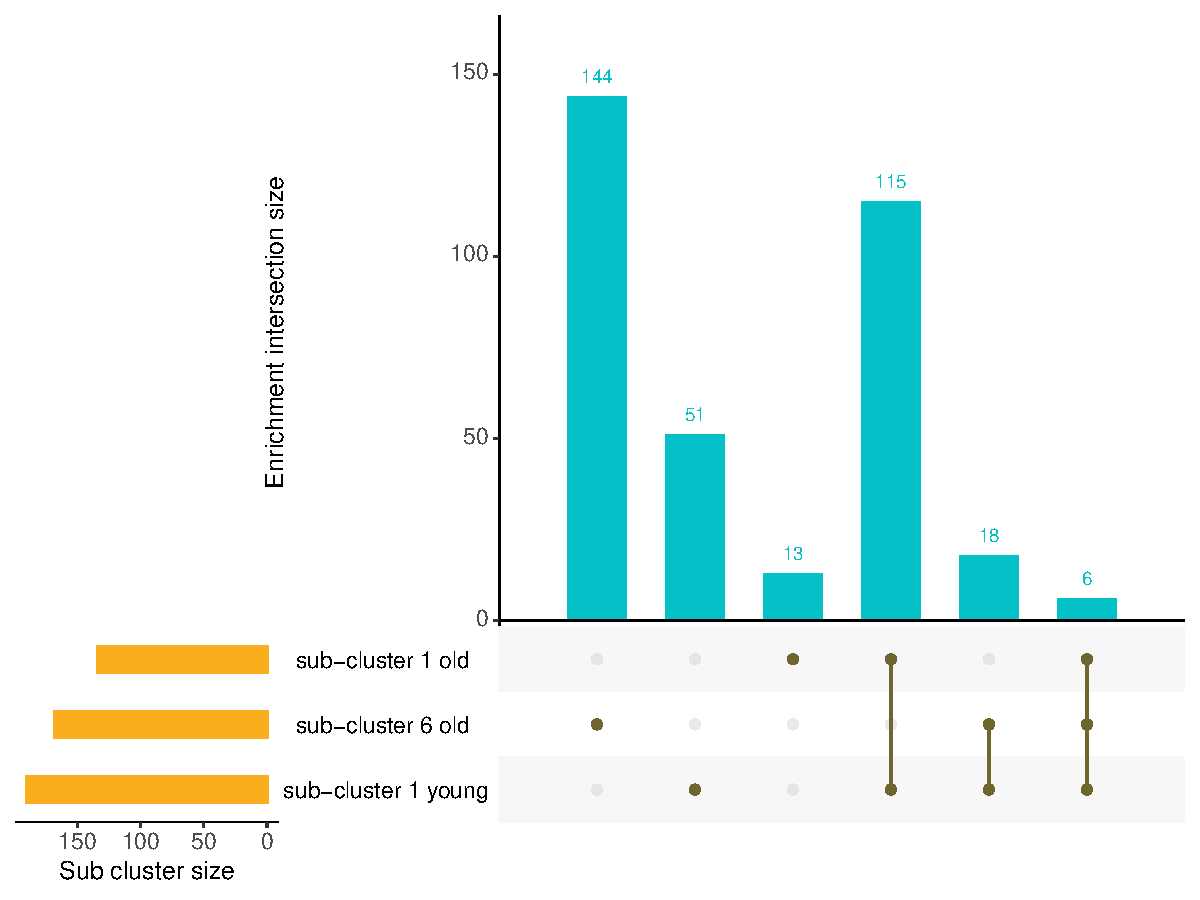
\includegraphics[width=\textwidth, center]{img/annexe_add_file_GWENA/additional_file_figure_5.pdf}
    \caption{Overlap between the enrichments found in sub-cluster 1 young, sub-cluster 1 old, and sub-cluster 6 old.(Upset diagram)}
    \label{fig:supp_fig_upset_subclusters_enrichments}
\end{figure} 


% \hfill \break
% \clearpage
% \bibliographystyle{unsrt}
% \bibliography{additional_file_1}